%% LyX 2.0.5.1 created this file.  For more info, see http://www.lyx.org/.
%% Do not edit unless you really know what you are doing.
\documentclass[usenatbib]{article}
\usepackage[latin9]{inputenc}
\usepackage[a4paper]{geometry}
\geometry{verbose}
\usepackage{color}
\usepackage{float}
\usepackage{graphicx}

\makeatletter

%%%%%%%%%%%%%%%%%%%%%%%%%%%%%% LyX specific LaTeX commands.
%% Because html converters don't know tabularnewline
\providecommand{\tabularnewline}{\\}
%% A simple dot to overcome graphicx limitations
\newcommand{\lyxdot}{.}


%%%%%%%%%%%%%%%%%%%%%%%%%%%%%% Textclass specific LaTeX commands.
\usepackage{jcappub}

%%%%%%%%%%%%%%%%%%%%%%%%%%%%%% User specified LaTeX commands.






%%%%%%%%%%%%%%%%%%%%%%%%%%%%%% LyX specific LaTeX commands.
%% A simple dot to overcome graphicx limitations
%Make my life significantly easier
\global\long\def\bd{{\bm{\delta}}}
\usepackage{astrobib_mnras2e}

\bibliographystyle{JHEP}

\makeatother

\begin{document}

\title{Generating Mock Catalogs for the Baryon Oscillation Spectroscopic
Survey: An Approximate N-Body approach}


\author{Tomomi Sunayama\textsuperscript{a}, Nikhil Padmanabhan\textsuperscript{a},
Katrin Heitmann\textsuperscript{b}, Salman Habib\textsuperscript{b},
Steve Rangel\textsuperscript{b,c}}


\abstract{Precision measurements of the large scale structure of the Universe
require large numbers of high fidelity mock catalogs to accurately
assess, and account for, the presence of systematic effects. We introduce
and test a scheme for generating mock catalogs rapidly using suitably
derated N-body simulations. Our aim is to reproduce the large scale
structure and the gross properties of dark matter halos with high
accuracy, while sacrificing the details of the halo's internal structure.
By adjusting global and local time-steps in an N-body code, we demonstrate
recovery of the relevant large scale probes, including individual
halo masses, to better than $2\%$ and the power spectrum to $k=1h{\rm Mpc^{-1}}$,
to better than $1\%$, while requiring a factor of 4 less CPU time.
To reduce the number of output snapshots, we also test the redshift
spacing of outputs required to generate simulated light cones. We
find that outputs separated by $\Delta0.05$ allow us to interpolate
particle positions and velocities with sufficient accuracy to reproduce
the real and redshift space power spectra to better than $1\%$ (out
to $k=1h{\rm Mpc^{-1}}$). Even with a redshift spacing as large as
$\Delta z=0.25$, these errors only degrade to less than $2\%$ in
both real and redshift space. As a practical demonstration of these
ideas, we generate a suit of simulations matched to the Baryon Oscillation
Spectroscopic Survey (BOSS).}


\affiliation{\textsuperscript{a}Yale University, New Haven, CT}


\affiliation{\textsuperscript{b }Argonne National Laboratory, Lemont, IL}


\affiliation{\textsuperscript{c }Northwestern University, Evanston, IL}


\emailAdd{tomomi.sunayama@yale.edu, nikhil.padmanabhan@yale.edu,heitmann@anl.gov,
habib@anl.gov,steverangel@u.northwestern.edu }


\keywords{cosmology; large-scale structure of Universe, cosmological parameters,
galaxies; halos, statistics}

\maketitle

\section{Introduction}

Large-volume spectroscopic surveys of the Universe (CITE SDSS, WiggleZ, BOSS)
are revolutionizing our understanding of cosmology and structure formation.
Based on these successes, a new generation of surveys (CITE DESI, Euclid, 
WFIRST) is being planned that will improve our constraints by an order
of magnitude (or more). This unprecedented improvement in statistical 
precision places stringent demands on the theoretical modeling and 
analysis techniques; simulations will play an essential in meeting these 
requirements. 

One of the challenges for simulations are the varied roles they play, 
and the different requirements these impose on the simulations. 
At one extreme, simulations are necessary for generating sample covariances 
for the data and measurements. This typically requires very large 
volumes to simulate entire surveys thousands of times, but have lower accuracy 
requirements. 
Motivated
by these considerations, a number of recent studies have investigated
methods designed to produce mock catalogs with reduced accuracy, but
much higher throughput compared to the full N-body
simulations~\cite{2002ApJ...564....8M,2002MNRAS.331..587M,2008MNRAS.391..435F,
2013AN....334..691R,2013arXiv1312.2013C,2013JCAP...06..036T,2014MNRAS.437.2594W,
2013MNRAS.433.2389M,2001A&A...367...18H,2009ApJ...701..945S,2014MNRAS.439L..21K,2014arXiv1409.1124C}.
An open question still is the effect of changing the input cosmology used
to generate the covariance matrix on cosmological inferences, and how 
best to implement such variations. More recently, the impact of super-survey
modes (modes outside the survey volume) on inferred errors has 
been shown to be potentially larger than previously appreciated (CITES??) 
and is an area of active study.

At the other extreme, simulations are crucial for calibrating the theoretical
models used to fit the data. Examples here are quantifying shifts in the
baryon acoustic oscillation distance scale due to nonlinear evolution
and galaxy bias (CITES), or templates used to fit the full shape of the 
correlation function. For such applications, one ideally requires 
high fidelity simulations. The volume requirements are significantly 
reduced from that for covariance matrices, but still need to much larger
than survey volumes to keep systematic errors below statistical errors.

An intermediate application are the generation of mock catalogs that capture
the observational characteristics of surveys (eg. geometry, selection 
effects). The importance of these cannot be underestimated, since the effects
of many observational systematics can only be quantitatively estimated 
by simulating them. These issues will get progressively more important
for the next generations of surveys which will move away from highly 
complete and pure samples that have mostly been used for cosmological studies 
to date.

The simplest way to generate approximate density fields is to use
analytic approximations such as Lagrangian perturbation theory followed
by prescriptions to put in halos in a way that better matches results
from N-body simulations~\cite{2013MNRAS.428.1036M,2014arXiv1401.4171M},
or simply to run lower resolution N-body codes with a small number
of time-steps~\cite{2013JCAP...06..036T}, or a combination of the
two approaches~\cite{2014MNRAS.437.2594W}. These methods are successful
in capturing the large-scale density field but lose information at
small scales. Because of their speed, they can be used to produce
large numbers of simulations required to build sample covariance matrices,
at error levels ranging from $5-10\%$ (depending on the quantities
being predicted). It is difficult to estimate, however, what the loss
of accuracy implies for tests of systematic errors, which may need
to be modeled at the $\sim1\%$ level.

The approach we take here is to reduce the small-scale accuracy of
a high-resolution N-body code by coarsening its temporal resolution.
In the present case, the time-stepping consists of two components,
(i) a long time step for solving for evolution under the long-range
particle-mesh (PM) force, and (ii) a set of underlying sub-cycled
time steps for a short-range particle-particle interaction, computed
either via a tree-based algorithm, or by direct particle-particle
force evaluations. The idea is to reduce the number of both types
of time steps while preserving enough accuracy to correctly describe
the large scale distribution of galaxies, as modeled by a halo occupation
distribution (HOD) approach. 
Our first goal in this paper is, therefore, to quantitatively understand
the impact of the temporal resolution on the halo density field and
how best to 
accurately reproduce the details of the halo density field on large
scales, sacrificing small scale structure information. 
This allows to generate a suite of large volume simulations, spanning
a range of cosmologies. This paper presents the details of these simulations
and outlines future applications.

This paper is organized as follows. Sec.~2 briefly describes the Hardware/Hybrid
Accelerated Cosmology Code (HACC) N-body framework we use to generate our
simulations, focusing on the flexibility in the time-stepping that we exploit here. 
Sec.~3 presents a sequence of convergence tests where we evaluate the effects
of time-stepping on the halo density field. Sec.~4 discusses interpolating between
saved time steps, necessary for constructing light-cone outputs. Sec.~5 presents
an example application of these simulations : generating mock catalogs that 
match the BOSS galaxy sample. (NOTE : Can we put in another simple application?) 
We conclude in Sec.~6 by outlining possible future directions.

All simulations and calculations in this paper assume a $\Lambda$CDM
cosmology with $\Omega_{m}=0.2648$, $\Omega_{\Lambda}=0.7352$, $\Omega_{b}h^{2}=0.02258$,
$n_{s}=0.963$, $\sigma_{8}=0.8$ and $h=0.71$.

%%\section{Introduction}
%%
%%Large-volume spectroscopic surveys of the Universe have revolutionized
%%our knowledge of structure formation and have established unprecedented
%%levels of statistical error in measuring various aspects of galaxy
%%clustering. Because of the demands on precision and accuracy imposed
%%by observational campaigns that seek to investigate the nature of
%%cosmic acceleration, the requirements on synthetic or mock catalogs
%%designed to test and validate survey methodologies, have also become
%%very severe. For many applications, such as to the Baryon Oscillation
%%Spectroscopic Survey (BOSS)~\cite{2013AJ....145...10D} and the near-future
%%Dark Energy Spectroscopic Instrument (DESI) project, a large number
%%of high-precision mock catalogs are needed. In order to encompass
%%the survey volume, such catalogs can only be created by running large-volume,
%%computationally expensive, N-body simulations. A large number of simulations
%%-- with varying cosmological parameters -- may be required in order
%%to assess systematic effects and to estimate error covariances. Motivated
%%by these considerations, a number of recent studies have investigated
%%methods designed to produce mock catalogs with reduced accuracy, but
%%much higher throughput compared to the full N-body simulations~\cite{2002ApJ...564....8M,2002MNRAS.331..587M,2008MNRAS.391..435F,2013AN....334..691R,2013arXiv1312.2013C,2013JCAP...06..036T,2014MNRAS.437.2594W,2013MNRAS.433.2389M,2001A&A...367...18H,2009ApJ...701..945S,2014MNRAS.439L..21K,2014arXiv1409.1124C}.
%%Many of these efforts have focused on error covariances, which allow
%%for significantly degraded error tolerances. Here, we are concerned
%%with the task of generating mock catalogs at levels of error control
%%that are similar to the level at which different N-body codes might
%%deviate, in other words, we seek to maintain close to state of the
%%art error tolerances in the quantities relevant for generating mock
%%catalogs. The aim is to keep these error tolerances lower than the
%%level of statistical error in the actual observations.
%%
%%The simplest way to generate approximate density fields is to use
%%analytic approximations such as Lagrangian perturbation theory followed
%%by prescriptions to put in halos in a way that better matches results
%%from N-body simulations~\cite{2013MNRAS.428.1036M,2014arXiv1401.4171M},
%%or simply to run lower resolution N-body codes with a small number
%%of time-steps~\cite{2013JCAP...06..036T}, or a combination of the
%%two approaches~\cite{2014MNRAS.437.2594W}. These methods are successful
%%in capturing the large-scale density field but lose information at
%%small scales. Because of their speed, they can be used to produce
%%large numbers of simulations required to build sample covariance matrices,
%%at error levels ranging from $5-10\%$ (depending on the quantities
%%being predicted). It is difficult to estimate, however, what the loss
%%of accuracy implies for tests of systematic errors, which may need
%%to be modeled at the $\sim1\%$ level.
%%
%%The approach we take here is to reduce the small-scale accuracy of
%%a high-resolution N-body code by coarsening its temporal resolution.
%%In the present case, the time-stepping consists of two components,
%%(i) a long time step for solving for evolution under the long-range
%%particle-mesh (PM) force, and (ii) a set of underlying sub-cycled
%%time steps for a short-range particle-particle interaction, computed
%%either via a tree-based algorithm, or by direct particle-particle
%%force evaluations. The idea is to reduce the number of both types
%%of time steps while preserving enough accuracy to correctly describe
%%the large scale distribution of galaxies, as modeled by a halo occupation
%%distribution (HOD) approach. Our first goal in this paper is, therefore,
%%to accurately reproduce the details of the halo density field on large
%%scales, sacrificing small scale structure information. Our second
%%goal is to build a set of simulations and related mock catalogs suitable
%%for BOSS analyses.
%%
%%In the following, we first briefly describe the methodology behind
%%relaxing the resolution of the N-body simulations. In Section 3, we
%%test and compare our method against results from the full N-body simulation
%%and explain how we calibrate our samples. In Sections 4 and 5, we
%%build a light cone output, populate halos in our samples with galaxies,
%%and compute correlation functions based on BOSS Data Release 11.
%%
%%All simulations and calculations in this paper assume a $\Lambda$CDM
%%cosmology with $\Omega_{m}=0.2648$, $\Omega_{\Lambda}=0.7352$, $\Omega_{b}h^{2}=0.02258$,
%%$n_{s}=0.963$, $\sigma_{8}=0.8$ and $h=0.71$.
%%

\section{HACC}

All simulations in this paper were carried out using the HACC (Hardware/Hybrid
Accelerated Cosmology Code) framework. HACC provides an advanced,
architecture-agile, extreme-scale N-body capability targeted to cosmological
simulations. It is descended from an approach originally developed
for the heterogeneous architecture of Roadrunner \cite{1742-6596-180-1-012019,Pope:2010:AU:1845737.1845828},
the first computer to break the petaflop performance barrier.

HACC's flexible code architecture combines MPI with a variety of more
local programming models, (e.g., OpenCL, OpenMP) and is easily adaptable
to different platforms. HACC has demonstrated scaling on the entire
IBM BG/Q Sequoia system up to 1,572,864 cores with an equal number
of MPI ranks, attaining 13.94 PFlops at 69.2\% of peak and 90\% parallel
efficiency (for details, see Ref.\cite{2012arXiv1211.4864H}). Examples
of science results obtained using HACC include 64-billion particle
runs for baryon acoustic oscillations predictions for the BOSS Lyman-$\alpha$
forest \cite{2010ApJ...713..383W}, high-statistics predictions for
the halo profiles of massive clusters \cite{2013ApJ...766...32B},
and 0.5 and 1.1~trillion particle runs at high mass resolution. A
recent overview of the HACC framework can be found in Ref.~\cite{hacc_2014}.

HACC uses a hybrid parallel algorithmic structure, splitting the force
calculation into a specially designed grid-based long/medium range
spectral PM component that is common to all computer architectures,
and an architecture-specific short-range solver. Modular code design
combined with particle caching allows the short-range solvers to be
`hot-swappable' on-node; they are blind to the parallel implementation
of the long-range solver. The short-range solvers can use direct particle-particle
interactions, i.e., a P$^{3}$M algorithm \cite{1988csup.book.....H},
as on (Cell or GPU) accelerated systems, or use tree methods on conventional
or many-core architectures. (This was the case for the simulations
reported here.) In all cases, the time-stepping scheme is based on
a symplectic method with (adaptive) sub-cycling of the short-range
force. The availability of multiple algorithms within the HACC framework
allows us to carry out careful error analyses, for example, the P$^{3}$M
and the TreePM versions agree to within $0.1\%$ for the nonlinear
power spectrum test in the code comparison suite of Ref.~\cite{2005ApJS..160...28H}.

As already discussed, an important feature of the work presented here
is the ability to carry out error-controlled approximate simulations
at high throughput. In order to understand how we implement this,
some details of the HACC time-stepping algorithm are now provided.
Evolution is viewed as a symplectic map on phase space: $\zeta(t)=\exp(-t{\bf {H}})\zeta(0)$
where, $\zeta$ is a phase-space vector $({\bf x},{\bf v})$, $H$
is the (self-consistent) Hamiltonian, and the operator, ${\bf {H}}=[H,~]_{P}$,
denotes the action of taking the Poisson bracket with the Hamiltonian.
Suppose that the Hamiltonian can be written as the sum of two parts;
then by using the Campbell-Baker-Hausdorff (CBH) series we can build
an integrator for the time evolution; repeated application of the
CBH formula yields 
\[
\exp(-t({\bf {H}}_{1}+{\bf {H}}_{2}))=\exp(-(t/2){\bf {H}}_{1})\exp(-t{\bf {H}}_{2})\exp(-(t/2){\bf {H}}_{1})+O(t^{3}),
\]
a second order symplectic integrator. In the basic PM application,
the Hamiltonian $H_{1}$ is the free particle (kinetic) piece while
$H_{2}$ is the one-particle effective potential; corresponding respectively
to the `stream' and `kick' maps $M_{1}=\exp(-t{\bf {H}}_{1})$ and
$M_{2}=\exp(-t{\bf {H}}_{2})$. In the stream map, the particle position
is drifted using its known velocity, which remains unchanged; in the
kick map, the velocity is updated using the force evaluation, while
the position remains unchanged. This symmetric `split-operator' step
is termed SKS (stream-kick-stream). A KSK scheme constitutes an alternative
second-order symplectic integrator.

In the presence of both short and long-range forces, we split the
Hamiltonian into two parts, $H_{1}=H_{sr}+H_{lr}$ where $H_{sr}$
contains the kinetic and particle-particle force interaction (with
an associated map $M_{sr}$), whereas, $H_{2}=H_{lr}$ is just the
long range force, corresponding to the map $M_{lr}$. Since the long
range force varies relatively slowly, we construct a single time-step
map by sub-cycling $M_{sr}$: $M_{full}(t)=M_{lr}(t/2)(M_{sr}(t/n_{c}))^{n_{c}}M_{lr}(t/2)$,
the total map being a usual second-order symplectic integrator. This
corresponds to a KSK step, where the S is not an exact stream step,
but has enough $M_{sr}$ steps composed together to obtain the required
accuracy. (We take care that the time-dependence in the self-consistent
potential is treated correctly; HACC uses the scale factor, $a$,
as the time variable.) As discussed later below, we will use the flexibility
in the sub-cycling as a way of reducing the number of time steps such
that the loss of accuracy only affects the resolution at very small
scales, which, as discussed previously, are not of interest in the
current set of simulations.


\section{Time Step Tuning}

In this section, we systematically examine how reducing the number
of time steps affects individual halo properties (i.e., halo masses,
positions, and velocities), as well as aggregate statistics like the
mass function and spatial clustering. We run a set of convergence
tests with boxes of size $(256h^{-1}{\rm Mpc})^{3}$ with $256^{3}$
particles. These runs have the same particle mass as the main $(4000h^{-1}{\rm Mpc})^{3}$
volume simulations. We run these with the following time step options
: 450/5, 300/3, 300/2, 150/3 and 150/2 where the first number is the
number of long time-steps, while the second is the number of subcycles.
The 450/5 case has been independently verified to give fully converged
results and is the baseline against which we compare all other results.
Each simulation is started from the same initial conditions and evolved
down to $z=0.15$. We demonstrate that the 300/2 case, corresponding
to $\Delta a\approx0.003$ reproduces the full resolution simulation
for all the large scale properties we consider, and is our choice
for the mocks presented in Sec.~5.


\subsection{Matching }

In order to compare detailed halo properties we need to match individual
halos across different runs (reference vs. run under test). We first
discuss the algorithm used for identifying the corresponding halos
in the two cases and then compare halo mass, position, and velocity
for the matched halos. From this quantitative comparison, we find
that the simulations with 300 global time steps have significantly
less scatter in the measured quantities, compared to the baseline
determined by the 450/5 simulation, than do the samples with 150 global
steps. In addition, we find that the differences between the different
sub-cycling choices are almost negligible.


\subsubsection{Algorithm}

All simulations share the same particle initial conditions, allowing
us to match halos in different runs by matching their individual particle
content. Given a halo in simulation A, we consider all halos in simulation
B that between them hold all the particles belonging to the halo in
simulation A. Given this list of possible matches, we choose the run
B halo with the largest number of common particles with the reference
halo in run A. To avoid spurious matches, we also require that the
fraction of common particles (relative to simulation A) exceeds a
given threshold. To illustrate how this matching algorithm works,
we use the samples from the 300/2 simulation and the 450/5 simulation,
and adopt a threshold of 50\% as our default choice. (Figure \ref{fig:mass-content}
demonstrates that the unmatched fraction increases with increasing
threshold and decreasing halo mass.)

\begin{figure}[H]
\includegraphics[width=0.5\columnwidth]{\lyxdot \lyxdot /Plots/unmatchHalo2_content_300_2_z0\lyxdot 15}

\caption{\label{fig:mass-content} Itemization of unmatched halos (from the
450/5 and 300/2 simulations at $z=0.15$) shown as cumulative number
densities of the unmatched halos arising from each procedure in the
matching algorithm. The solid blue line is the total number density
of the unmatched halos. The dashed green line shows halos with no
counterpart -- none of the particles were identified as belonging
to a halo in the comparison simulation; this is significant only at
low halo mass. The dashed red line shows halos eliminated because
of not meeting the matching threshold (i.e., the halos do not have
enough of a fraction of the same particles). The dashed cyan line
is for the halos eliminated because multiple halos correspond to one
halo (see text). }
\end{figure}


The matching algorithm described above is unidirectional, hence multiple
halos in run A may have particles resident in a single halo in run
B; in our simulations, this happens at the 1-2\% level, adopting a
particle matching threshold of 50\%. We refer to these cases as `multiply-booked'
halos. Figure~\ref{fig:mass-scatter1} compares halo masses matching
the 450/5 simulation to the 300/2 simulation for the case of multiply-booked
halos, as well as the rest. The top left panel shows the mass scatter
for all the matched halos between the two simulations, while the top
right panel shows the mass scatter only for the non multiply-booked
halos. The bottom panels show the mass scatter for the case of multiply-booked
halos only. The bottom left panel shows the mass scatter for individual
multiply-booked halos, while the bottom right panel plots the summed
halo mass for the corresponding halos. The overall behavior represented
in Figure~\ref{fig:mass-scatter1} is straightforward to interpret.

\begin{figure}[h]
\includegraphics[width=0.465\columnwidth]{\lyxdot \lyxdot /Plots/testDB_mass_300_2_z0\lyxdot 15}
\includegraphics[width=0.535\columnwidth]{\lyxdot \lyxdot /Plots/testDB_nonDB_300_2_z0\lyxdot 15}

\includegraphics[width=0.465\textwidth]{\lyxdot \lyxdot /Plots/testDB_DB_numPartCut_300_2_z0\lyxdot 15}
\includegraphics[width=0.535\columnwidth]{\lyxdot \lyxdot /Plots/testDB_sum_mass_f0\lyxdot 5_300_2_z0\lyxdot 15}

\caption{\label{fig:mass-scatter1}Distribution of halo masses comparing matched
halos in the 450/5 simulation (x-axis) to the 300/2 simulation (y-axis)
at $z=0.15$. Panels correspond to halos with different matching criteria
imposed: all the matched halos (top left), the vast majority of matched
halos having one-to-one correspondence (top right), matched halos
not having one-to-one correspondence called ``multiply-booked''
halos (bottom left), and the multiply-booked halos whose corresponding
halo masses are added (bottom right). The results shown in these panels
imply that the low-mass scatter between the 450/5 simulation and the
300/2 simulation shown in the top left panel arises when``multiply-booked''
halos in the 450/5 simulation are merged into one halo in the 300/2
simulation due to an effectively worse resolution in this case.}
\end{figure}


As the top left panel shows, there are low-mass halos in the 450/5
simulation corresponding to high-mass halos in the 300/2 simulation.
The same trend is observed for the case of multiply-booked halos (bottom
left panel), but not for the non-multiply-booked halos (top right).
Furthermore, the disagreement for halo masses between the two simulations
are resolved by adding the corresponding halo masses. This implies
that there are multiple halos in the 450/5 simulation which are merged
into one halo in the 300/2 simulation. The smaller number of time
steps in the 300/2 simulations reduces substructure as well as the
compactness of the halos compared to the 450/5 simulation. Thus, for
a small fraction of halos in the 450/5 simulation, individual halos
can be merged into a single halo in the 300/2 simulation.

Figure \ref{fig:mass-content} shows the number densities of the unmatched
halos in the 450/5 simulation when compared to the 300/2 simulation
at $z=0.15$. There are three reasons that halos can turn up as unmatched.
In the first case, particles forming a halo in simulation A may not
form a component of a halo in simulation B (no common particles).
Second, if the fraction of common particles over the total number
of particles in each halo is less than the threshold of 50\%, these
halos will be eliminated from the matching set. Finally, for the case
of multiply-booked halos, we remove all but the one with the largest
number of common particles. In Figure \ref{fig:mass-content}, we
show each type of unmatched number density as a function of halo mass.
The first case occurs only for low halo masses, where low effective
resolution in a simulation can lead to halo drop out (halos are too
'fuzzy' to meet the FOF overdensity criterion), and falls off steeply
with rising halo mass. Most of the unmatched halos arise due to their
not passing the threshold criterion. The loss of matching due to multiple-booking
follows the trend of the below-threshold case, but at a reduced level.
We have checked that the trends discussed here are not affected by
redshift.


\subsubsection{Halo Properties}

We now systematically compare halo properties (i.e., halo mass, position,
and velocity) for halos in the lower resolution runs that were successfully
matched to those in the 450/5 simulation. We are interested in correctly
describing the large-scale distribution of galaxies using an HOD approach;
this requires that only the dark matter halo locations and masses
be estimated sufficiently accurately.

The comparison of halo mass for different time-stepping schemes to
the 450/5 simulation at $z=0.15$ is shown in Figure \ref{fig:HaloProperty_mass}.
We take all the matched halos whose masses are between $10^{12.5}{\rm M_{\odot}}$
to $10^{13.0}{\rm M_{\odot}}$, $10^{13.0}{\rm M_{\odot}}$ to $10^{13.5}{\rm M_{\odot}}$,
and $10^{13.5}{\rm M_{\odot}}$ to $10^{14.0}{\rm M_{\odot}}$, and
compute their means and standard deviations for ${\rm log_{10}(M/M_{450/5})}$,
where $M_{450/5}$ is a halo mass for the 450/5 simulation and $M$
corresponds to a halo in the samples generated with different time-stepping
schemes. Figure \ref{fig:HaloProperty_mass} shows that halos generated
from the simulations with small number of time steps have systematically
lower FOF masses than those in the 450/5 simulation. (The same linking
length ($b=0.168$) is used in the FOF algorithm to define halos for
all the simulations.) Under these circumstances, the FOF mass is highest
in the 450/5 simulation, decreasing systematically with increase in
loss of temporal resolution.

\textcolor{red}{NOTE: because FOF masses come from particles within
an isodensity contour, it is not obvious that making the resolution
worse will actually reduce the mass -- it can even increase the mass,
depending on the circumstances (see Bhattacharya et al. arXiv:1005.2239,
the Appendix)}

\begin{figure}[h]
\textcolor{black}{\includegraphics[width=0.5\columnwidth]{\lyxdot \lyxdot /Plots/massSlice_z0\lyxdot 15}}

\textcolor{black}{\caption{\label{fig:HaloProperty_mass}Comparison of halo mass (FOF, $b=0.168$)
for matched halos between the 450/5 simulation and coarsened time-stepping
schemes at $z=0.15$. We take all the matched halos whose masses are
between $10^{12.5}{\rm M_{\odot}}$ to $10^{13.0}{\rm M_{\odot}}$,
$10^{13.0}{\rm M_{\odot}}$ to $10^{13.5}{\rm M_{\odot}}$, and $10^{13.5}{\rm M_{\odot}}$
to $10^{14.0}{\rm M_{\odot}}$, and compute the mean and the standard
deviation for ${\rm log_{10}(M/M_{450/5})}$ where $M_{450/5}$ is
a halo mass for the 450/5 simulation and $M$ is for the simulations
with different number of time steps corresponding to different colors
in the plot. The x-positions have been displaced to avoid overlapping
the error bars. Halo masses decrease systematically as the time resolution
is coarsened.}
}
\end{figure}


Figure~\ref{fig:HaloProperty_step} shows the differences in positions
(left panel) and velocities (right panel) for the matched halos at
$z=0.15$. Simulations with a smaller number of global time steps
(150) display significantly more scatter; they also show a small bias
in the speed. With 300 global time steps, the results are much improved;
the velocity bias is almost entirely removed and the scatter is significantly
reduced. The standard deviation in the differences in halo distances
is matched is better than $200h^{-1}{\rm kpc}$ in these cases. \textcolor{black}{The
distributions are very close to Gaussian. }As is clear from Figure~\ref{fig:HaloProperty_step},
the difference between 3 and 2 sub-cycles is insignificant for our
purposes. We observe the same trend in halo properties discussed here
at different redshifts.

As shown in Figure \ref{fig:mass-content}, the fraction of unmatched
halos in the 300/2 simulation to the 450/5 simulation is less than
$5\%$ on most of halo mass ranges, which implies that the 300/2 simulation
has almost the same number of halos as in the 450/5 simulation. Furthermore,
Figure \ref{fig:mass-scatter1} shows that the halo masses in the
450/5 and 300/2 simulations have linear relation with the slope being
one. So, most of halos in the 300/2 simulation have the same mass
as the ones in the 450/5 simulation. Since the number of sub-cycles
do not affect to halo positions and velocities as shown in Figure
\ref{fig:HaloProperty_step}, the 300/2 time step is our choice to
save the simulation time while keeping the halo properties almost
identical to the 450/5 simulation.

\begin{figure}[h]
\includegraphics[width=0.5\columnwidth]{\lyxdot \lyxdot /Plots/histogram_x_z0\lyxdot 15}\includegraphics[width=0.5\columnwidth]{\lyxdot \lyxdot /Plots/histogram_vx_z0\lyxdot 15}

\caption{\label{fig:HaloProperty_step}Comparison of the positions (left) and
velocities (right) of halos matched across simulations with different
time steps. The reference simulation is 450/5 while the colors correspond
to 300/3 (blue), 300/2 (green), 150/3 (red), and 150/2 (cyan). The
dashed lines are Gaussian fits.}
\end{figure}


The results shown in Figures~\ref{fig:mass-content}, \ref{fig:mass-scatter1},
and \ref{fig:HaloProperty_step}, show that the the 300/2 option has
a low ratio of unmatched halos (less than $5\%$), excellent halo
mass correlation to the 450/5 simulation (the small mass bias can
be easily corrected as described below), and sufficiently small scatter
in halo position. This time-stepping option is therefore a good candidate
for generating mock catalogs efficiently, while maintaining high accuracies.
In terms of the time savings alone, this will result in an increased
capacity to generate high quality catalogs by a factor of four, which
is quite significant. We will consider memory and storage savings
further below in Section~4.


\subsubsection{Halo Mass Adjustment and Resulting Observables}

Halos generated by the de-tuned simulations have systematically lower
masses than the halos in the 450/5 simulation as shown in Figure~\ref{fig:HaloProperty_mass}.
In the following, we describe how to implement a systematic mass correction
by matching to the 450/5 results; we also display the resulting observables
including mass functions and power spectra.

To undertake the mass calibration, we first take all the matched halos
between the 450/5 simulation and the de-tuned simulations and compute
means for each mass bin. We consider only the matched halos because
the aim of the mass adjustment is to correct systematic mass differences
for the halos that are theoretically identical in the different runs.
After computing the means for each mass bin, we fit them to a functional
form that brings the reassigned halo mass, $M_{re}$, close to the
average halo mass for the 450/5 simulation. For our simulations, we
find that the following simple form suffices for this task:

\begin{equation}
M_{re}=M(1.0+\alpha(M/10^{12.0}[{\rm M_{\odot}])^{\beta},}\label{eq:mass_adjust}
\end{equation}
where $M_{re}$ is the reassigned halo mass, $M$ is the original
halo mass, and $\alpha$ and $\beta$ are free parameters. The $\alpha$
and $\beta$ values for the simulations with different numbers of
time steps are listed in Table \ref{tab:free_param1} (at $z=0.15$).
The best-fit parameters $\alpha$ and $\beta$ are functions of redshift.
For the case of the 300/2 simulation, the best fit parameters are
$\alpha(z)=0.123z+0.052$ and $\beta(z)=-0.154z-0.447$.

\begin{table}
\begin{tabular}{|c|c|c|}
\hline 
 & $\alpha$  & $\beta$\tabularnewline
\hline 
\hline 
300/3  & 0.005  & 0.175\tabularnewline
\hline 
300/2  & 0.07  & -0.47\tabularnewline
\hline 
150/3  & 0.101  & -0.162\tabularnewline
\hline 
150/2  & 0.315  & -0.411\tabularnewline
\hline 
\end{tabular}

\caption{\label{tab:free_param1}Mass reassignment parameters $\alpha$ and
$\beta$ of Eq.~\ref{eq:mass_adjust} for simulations run with different
numbers of time steps (the results are shown at $z=0.15$).}
\end{table}


Given the mass corrections, we now compute mass functions using the
results from the different time-stepping schemes, as shown in Figure~\ref{fig:massFn_step},
where we use the 450/5 simulation at $z=0.15$ as the reference. In
Figure \ref{fig:massFn_step}, we show the ratio $n(>M)/n_{450/5}(>M)$,
where $n_{450/5}(>M)$ is a cumulative mass function for the 450/5
simulation and $n(>M)$ is a cumulative mass function for the other
cases. We compare the results before and after mass adjustment. While
the mass functions from the 250/3 and 150/2 simulations are suppressed
by more than 10\% on all mass ranges before correction, they are significantly
improved afterwards, especially for halo masses greater than $10^{13.0}{\rm M_{\odot}}$.
For simulations with 300 global time steps, the mass adjustment is
especially effective at small halo masses.

\begin{figure}[H]
\includegraphics[width=0.5\columnwidth]{\lyxdot \lyxdot /Plots/haloRatioNum256_z0\lyxdot 15}
\includegraphics[width=0.5\columnwidth]{\lyxdot \lyxdot /Plots/haloRatioNum256_tweak_z0\lyxdot 15}

\caption{\label{fig:massFn_step}Comparison of cumulative mass functions in
different simulations taking the 450/5 simulation as a reference.
Lines, from top to bottom, correspond to the time stepping choices,
300/3 (blue), 300/2 (green), 150/3 (red), and 150/2 (cyan) respectively.
The left panel shows the cumulative mass functions for unadjusted
masses (as described in the text), while the right panel shows the
post-correction results. A simple mass recalibration allows one to
successfully recover the mass functions, even in the extreme case
of the 150/2 simulation, for which the original result differed by
more than 10\% (on all mass scales). }
\end{figure}


We next compute the halo-matter cross power spectra between halo and
matter density fields in both real and redshift space, as shown in
Figure~\ref{fig:crossMater_step}. This figure shows the ratio $P_{hm}/P_{hm,450/5}$
at $z=0.15$, where $P_{hm,450/5}$ is the cross power spectrum for
the 450/5 simulation and $P_{hm}$ is the cross power spectrum for
other time steps. For the dark matter density field, we use the output
of the 450/5 simulation for all the halo samples. Note that the dark
matter density fields are in real-space for both cases. In this way,
the ratio $P_{hm}/P_{hm,450/5}$ in real-space is equivalent to the
ratio of halo bias between the 450/5 simulation and the simulations
with other time-steps. To select halos, we apply the soft-mass cut
method using the probability given by 
\begin{equation}
\langle N_{halo}(M)\rangle=\frac{1}{2}{\rm erfc}\left(\frac{{\rm log(M_{cut}/}M)}{\sqrt{2}\sigma}\right),
\end{equation}
where we set ${\rm M_{cut}=10^{13.0}[{\rm M_{\odot}]}}$ and $\sigma=0.5$.
This probability has a similar form to the HOD technique so that the
probability gradually becomes one as halo mass increases. We use this
method to avoid noise from halos scattering across sharp halo mass
boundaries. The errors calculated here are not due to sample variance
as we generate 10 samples from one full sample with the soft-mass
cut method. The results show that as the time stepping is coarsened,
the ratio of the cross power spectra increases, especially in redshift-space,
where we observe large deviations from unity on small scales for the
150/2 and 150/3 simulations. This is due to the overall smaller halo
velocities for those simulations, as shown in Figure~\ref{fig:HaloProperty_step}.
For the simulations with the 300 global time steps, overall agreement
with the 450/5 simulation is almost at the 1\% level on any scale
in both real-space and redshift-space. Based on these convergence
tests, we conclude that the 300/2 option meets the error requirements.

\begin{figure}[H]
\includegraphics[width=0.45\columnwidth]{\lyxdot \lyxdot /Plots/crossMatter_m450_tweak_softMcut13\lyxdot 0_s0\lyxdot 5_z0\lyxdot 15}\includegraphics[width=0.45\columnwidth]{\lyxdot \lyxdot /Plots/crossMatter_tweak256_redshift_z0\lyxdot 15}

\caption{\label{fig:crossMater_step} Ratio of halo-matter cross power spectra
as a function of time steps with respect to the 450/5 simulation at
$z=0.15$. We use the real-space halo density field for the left panel
and the redshift-space halo density field for the right panel; the
dark matter density fields used here are in real-space for both cases.
The left panel shows that agreements with the 450/5 simulation are
all within 2\%. In the right panel, the large discrepancy of the cross
power spectra for the simulations with 150 global steps on small scales
is mainly due to the systematically small velocities shown in Figure
\ref{fig:HaloProperty_step}. Note that the halos are selected based
on the soft mass-cut method with $M_{cut}=13.0$ and $\sigma=0.5$.}
\end{figure}



\section{Constructing Light Cones}

Once the simulations are run at the chosen time-stepping settings,
the next step is to construct light-cone outputs. Here, we build light
cones from snapshots whose redshift range is from $z=0.8$ to $z=0.15$,
with a constant redshift separation of $\Delta z=0.1$. The light
cone is constructed using spherical shells, each shell is centered
at the redshift of each snapshot, and has a redshift width of 0.1.
In each shell, we displace the halo positions by using their peculiar
velocities in order to shift to light cone positions:
\begin{equation}
\vec{x}|_{z=z_{pos}}=\vec{x}|_{z=z_{snap}}+\vec{v}_{pec}|_{z=z_{snap}}\Delta t,\label{eq:lightcone}
\end{equation}
where $z_{snap}$ is the redshift of the snapshot, $z_{pos}$ is the
redshift corresponding to its radial position, $\vec{v}_{pec}$ is
its peculiar velocity, and $\Delta t$ is the time elapsed between
$z_{snap}$ and $z_{pos}$. For the case of a halo crossing its boundary
of the shell, we choose the halo whose distance from the boundary
is closer before shifting.

To evaluate how shifting affects a spatial distribution of halos,
we compare the distances for the halos at different redshift before
and after shifting their positions. For the comparison, we use the
halos which exist at both redshifts by matching halo particle profiles,
which is the same method described in Section 3.1. Figure \ref{fig:Histograms-of-distance}
is the histograms of distances for the matched halos at $z=0.25$
and $z=0.15$ before and after shifting. After shifting halos, we
see that the mean distance between corresponding halos decreases from
$0.4h^{-1}{\rm Mpc}$to $0.1h^{-1}{\rm Mpc}$ and the standard deviation
shrinks from $0.2h^{-1}{\rm Mpc}$ to $0.1h^{-1}{\rm Mpc}$. This
result holds at all redshifts examined.

\begin{figure}[H]
\includegraphics[width=0.5\columnwidth]{\lyxdot \lyxdot /Plots/hist_dist_x_z0\lyxdot 25to0\lyxdot 15}

\caption{The histogram shown in blue is that of the distances between the position
of the halos at $z=0.25$ and where they have moved to in the simulation
at $z=0.15$. The histogram shown in green is that of the distances
between the positions of the halos at $z=0.15,$ and the positions
that would be predicted by shifting the positions from the $z=0.25$
simulation assuming the peculiar velocity was constant between the
snapshots (described in Eq. \ref{eq:lightcone}). The plot shows that
the distances between the halos at different redshifts become smaller
after the shifting. \label{fig:Histograms-of-distance}}
\end{figure}


As an additional check, we compare the affect on halo bias due to
shifting. Figure~\ref{fig:power-lightcone} shows the ratios of the
halo matter cross power spectra to an auto matter power spectrum at
$z=0.25$. The plot shows that shifting halos from $z=0.15$ to $z=0.25$
brings down the halo bias to the one at $z=0.25$ (an analogous test
is shown for redshifts $z=0.7$ and $z=0.8$). The agreement between
the original power spectrum at $z=0.25$ and the shifted power spectrum
is 99.8\% up to $k=1h{\rm Mpc^{-1}}$. This demonstrates that the
spatial distribution of the halos is statistically correct across
the scales of interest.
\begin{figure}[H]
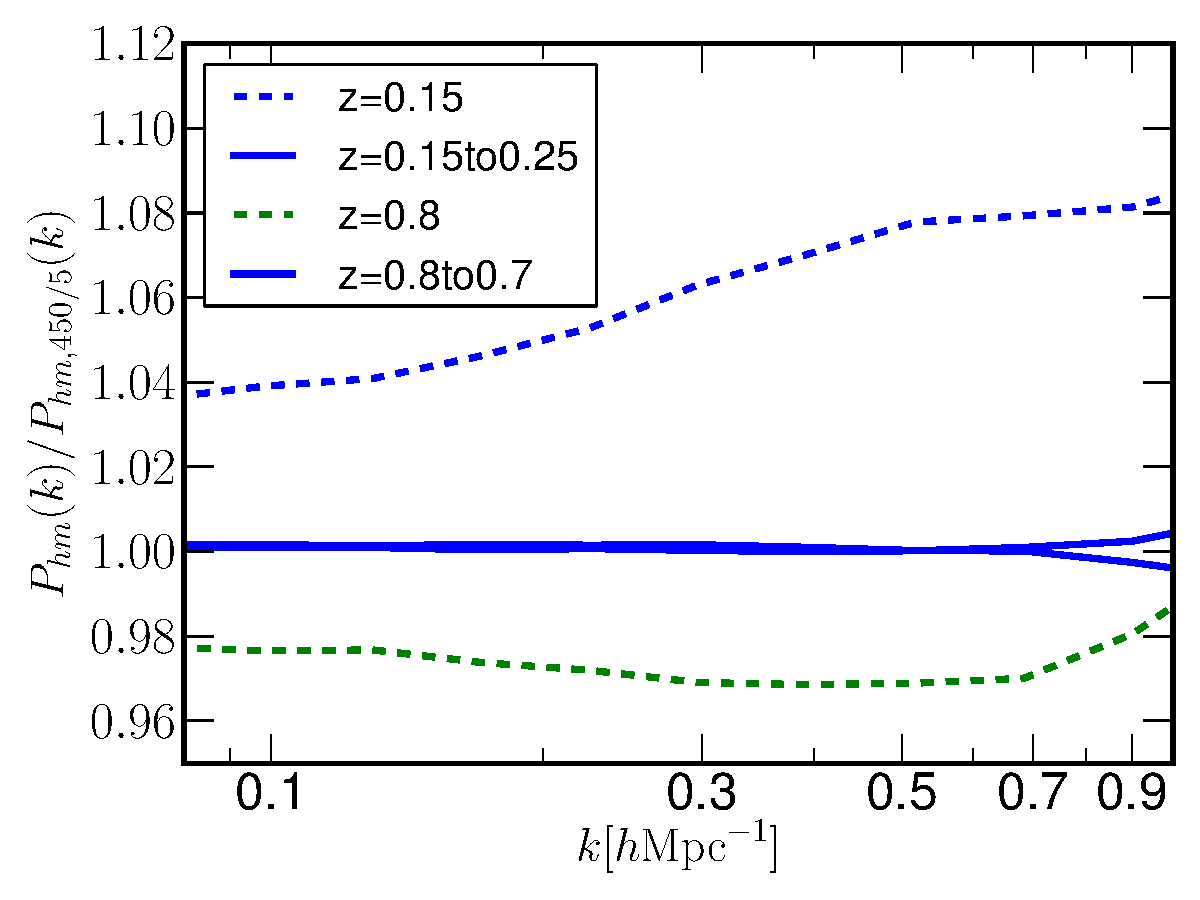
\includegraphics[width=0.5\columnwidth]{\lyxdot \lyxdot /Plots/shifting1}

\caption{\label{fig:power-lightcone}In this figure, we use the halo matter
cross power spectra at $z=0.25$ and $z=0.7$ as a denominator. The
dashed lines show the ratio with the cross power spectra at $z=0.15$
and $z=0.8$ respectively before shifting, and the solid lines are
the ratio after shifting halo positions. It indicates that shifting
the positions of halos from one redshift to the another preserves
the distribution of halos statistically.}
\end{figure}


A parameter when building light cones by stitching static snapshots
together is how large $\Delta z$ can be between various snapshots.
Figure \ref{fig:power-lightcone2} test this in both real and redshift
space; in redshift space, we assume the velocity of the object is
unchanged between the snapshots. We see that the agreement in real
space is within 1\% even for the case of shifting for $\Delta z=0.25$,
while the discrepancy increases more rapidly for larger $\Delta z$
in redshift space. In order to understand the cause of rapid discrepancy
of the power spectra in redshift-space, we further investigate the
distribution of velocity differences at different redshifts shown
in Figure \ref{fig:vel_hist_expFac}. We compare original velocities
computed from the simulations in the right panel, while we multiply
those velocity by the expansion factor $a(z)$ in the left panel.
By scaling with the expansion factor, the velocity differences at
different redshifts become smaller. Figure \ref{fig:shift-expFac}
shows the power spectra recomputed with the velocity multiplied by
the ratio of $a(z)/a(z=0.15)$, where $z$ is the redshift of the
simulation. The clustering in redshift-space is improved significantly
that the overall agreement becomes within 1\% on $k<1[h{\rm Mpc^{-1}]}$.

\textcolor{red}{NOTE: velocity scaling with scale factor ratio needs
to be justified --}

\begin{figure}[H]
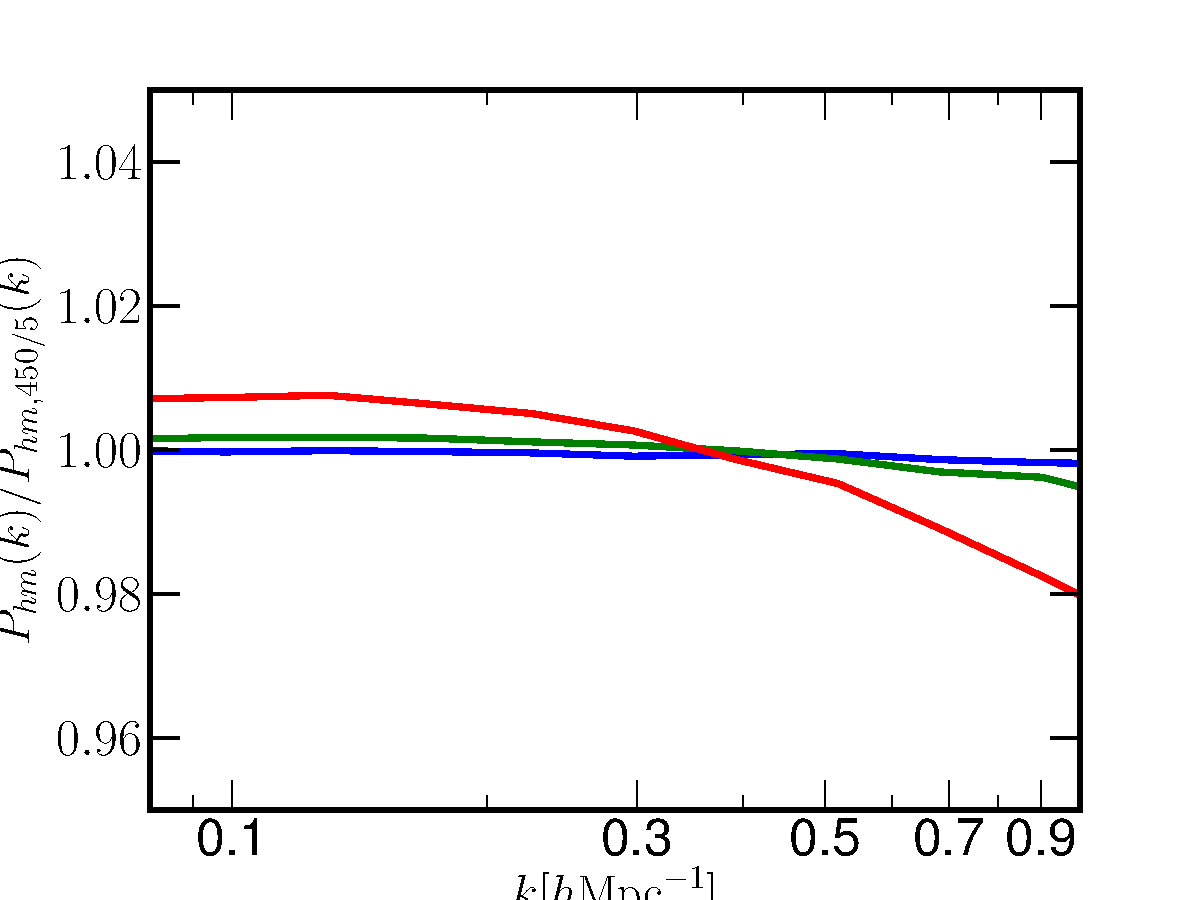
\includegraphics[width=0.5\columnwidth]{\lyxdot \lyxdot /Plots/test1}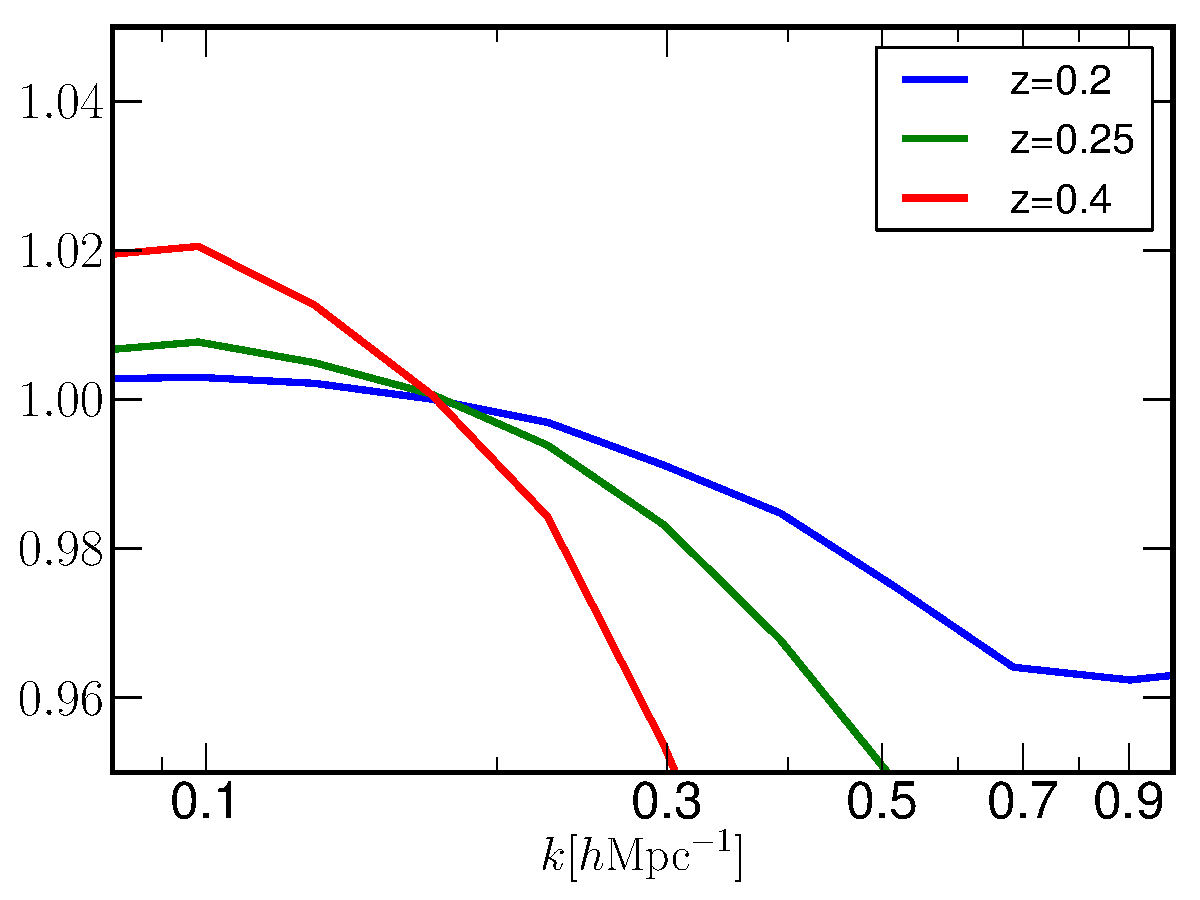
\includegraphics[width=0.5\columnwidth]{\lyxdot \lyxdot /Plots/test2}

\caption{\label{fig:power-lightcone2}Ratio of halo matter cross power spectra
in real space {[}left{]} and in redshift space {[}right{]} after shifting
the position of the halos from the redshift labeled in the plots to
$z=0.15$. The denominator is the cross power spectra at $z=0.15,$where
we use the halo density field in real space and redshift space respectively.
For all cases, we use the DM density field in real space at $z=0.15$. }
\end{figure}


\begin{figure}[H]
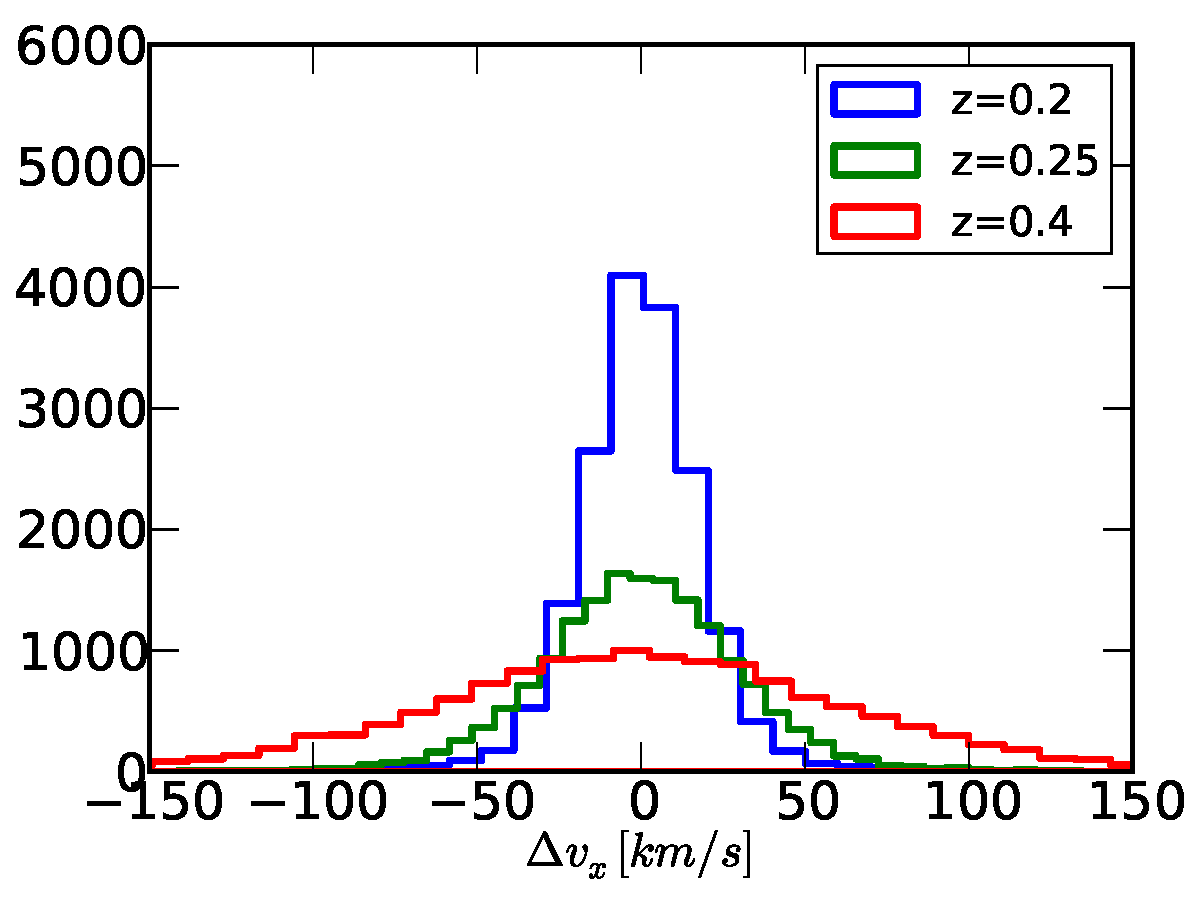
\includegraphics[width=0.5\columnwidth]{\lyxdot \lyxdot /Plots/hist_vx}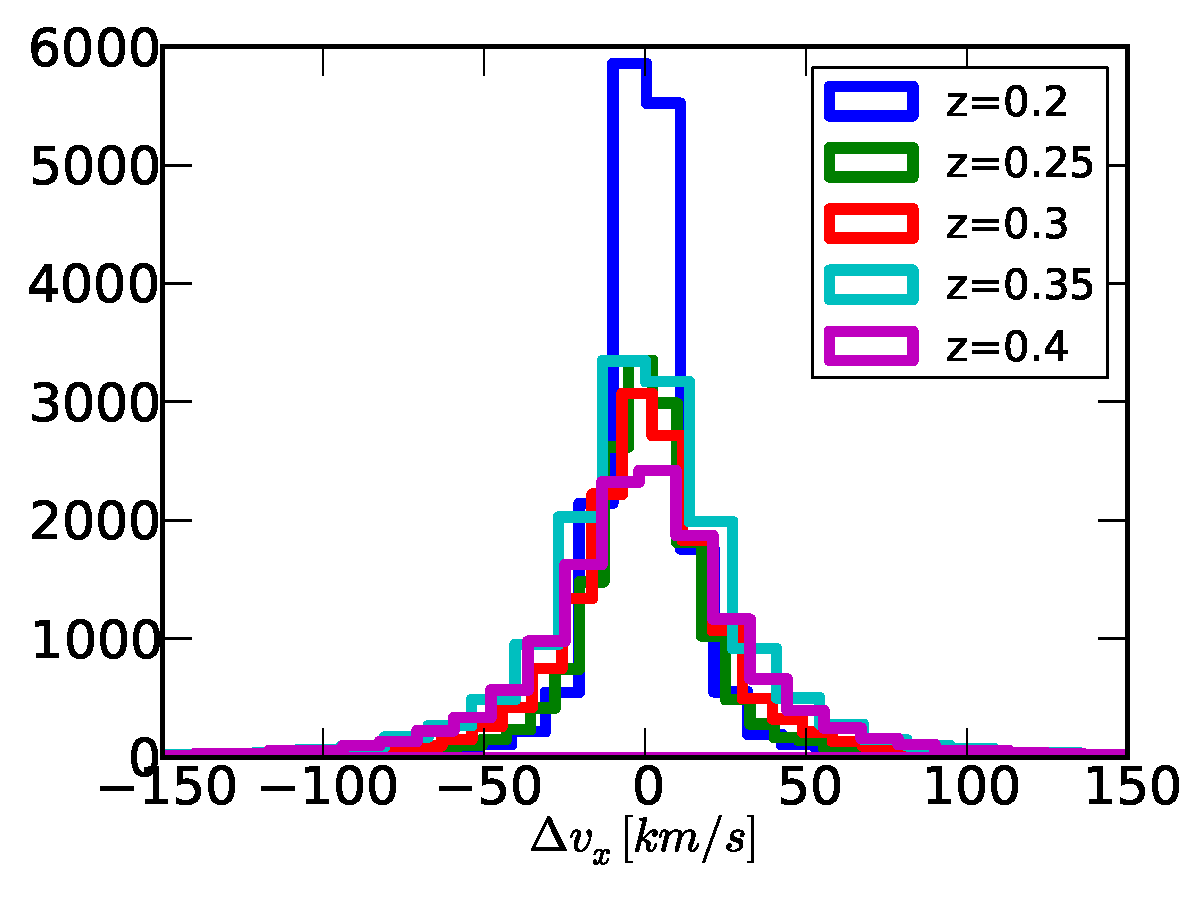
\includegraphics[width=0.5\columnwidth]{\lyxdot \lyxdot /Plots/hist_vx_expFac}

\caption{\label{fig:vel_hist_expFac}Comparisons of the velocities of halos
matched across simulations at different redshifts to the one at $z=0.15$.
From left to right, we compare original halo velocities and the velocities
multiplied by the expansion factor $a(z)$. As shown, the scatter
in the velocity differences decreases in the right panel. This indicates
that the change in velocities at different redshifts is largely affected
by the expansion of the Universe.}
\end{figure}


\begin{figure}
\includegraphics[width=0.5\columnwidth]{\lyxdot \lyxdot /Plots/shifting_s_expFac_z0\lyxdot 15}

\caption{\label{fig:shift-expFac}Ratio of halo matter cross power spectra
in redshift space as shown in Figure \ref{fig:power-lightcone2}.
The only difference is that here we use the velocity field multiplied
by the ratio of the expansion factor $a(z)/a(z=0.15)$ (where z is
the redshift shown in the figure) to compute the halo positions in
redshift-space. The denominator is the cross power spectra at $z=0.15,$where
we use the halo density field in redshift space. For all cases, we
use the DM density field in real space at $z=0.15$.}
\end{figure}



\section{BOSS Mock Catalogs}

As a concrete implementation of the approach discussed above, we construct
catalogs designed to mock BOSS galaxy samples. BOSS (\cite{2013AJ....145...10D}),
part of the SDSS-III project (\cite{2011AJ....142...72E}), is a spectroscopic
survey that aims to make percent level distance measurements using
the baryon acoustic oscillation technique. The low redshift ($z<0.7$)
distance measurements use two galaxy samples : the LOWZ ($z<0.45$)
and CMASS ($z<0.7$) samples (\cite{2014MNRAS.441...24A,2014MNRAS.440.2222T}).
We focus on the CMASS sample below; however, the same halo catalogs
are useful for the LOWZ sample as well.

We choose a simulation volume large enough to build a full-sky mock
BOSS catalog. Since the CMASS sample extends to $z\sim0.7$, we choose
a simulation side of $4000h^{-1}{\rm Mpc}$, corresponding to a comoving
distance to $z\sim0.8$ from the center of the box; Fig.~\ref{fig:boss-geom}
shows the BOSS CMASS redshift distribution as a function of redshift
and comoving distance (assuming our fiducial cosmology). Our simulations
are run with $4000^{3}$ particles, corresponding to a particle mass
of $10^{11}{\rm M_{\odot}}$. The characteristic halo mass for BOSS
galaxies corresponds to $10^{13}M_{\odot}$, which we resolve with
100 particles. We keep all halos down to 40 particles corresponding
to a halo mass of $10^{12.6}{\rm M_{\odot}}$. The simulations are
started at \textcolor{red}{$z=200$} with Zel'dovich initial conditions
and are stopped at $z=0.15$ with simulation outputs every $\Delta z=0.05$.
At each of these steps, we store \textcolor{red}{XXX}. 

\textcolor{red}{NOTE: complete final sentence -> This is for Salman
and Katrin to fill the details.}

The BOSS angular geometry is split into two regions : one in the North
Galactic Cap and one in the South Galactic Cap (Figure~\ref{fig:boss-geom}).
Since we generate full-sky mocks, it is straightforward to embed two
full non-overlapping BOSS surveys in a single mock realization (Figure~\ref{fig:boss-geom}).
We cut out a first BOSS volume with $\vec{x}_{old}$ and then define
a new coordinate system $\vec{x}_{new}$ such that $\vec{x}_{new}=R\vec{x}_{old}$,
where $R$ is the Euler rotation matrix for Figure~\ref{fig:boss-geom}:
\[
R=\left(\begin{array}{ccc}
0.088 & 0.096 & 0.991\\
0.219 & -0.973 & 0.075\\
0.972 & 0.211 & -0.107
\end{array}\right).
\]


\begin{figure}
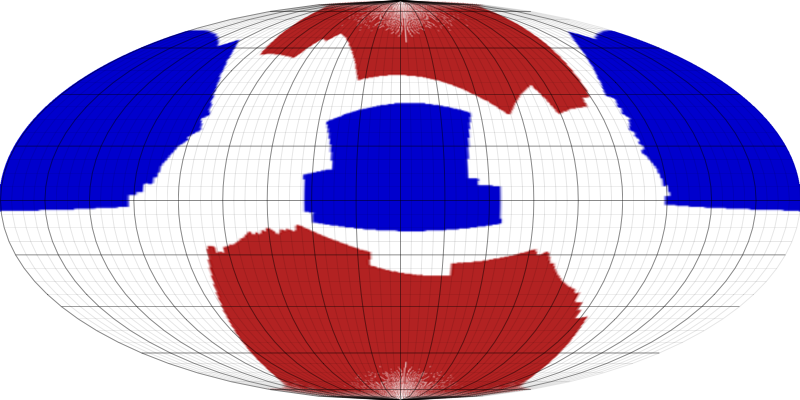
\includegraphics[width=0.5\columnwidth]{\lyxdot \lyxdot /Plots/boss_geom}

\caption{\label{fig:boss-geom}Fitting two non-overlapping BOSS volumes into
the same simulation box. The blue region is the BOSS survey footprint
in equatorial coordinates, while the red region is the same region
rotated using the rotation matrix given in the text.}
\end{figure}



\subsection{Building the Galaxy Catalog}

To generate the galaxy mock catalogs, we proceed in two steps, 1)
populate halos with galaxies using an HOD approach, 2) assign positions
and velocities to the galaxies assuming an NFW profile~\cite{1996ApJ...462..563N}.
The HOD functional form (based on a number of free parameters, 5 in
our case) provides probabilities for the number of central and satellite
galaxies based on the masses of halos that host those galaxies. A
halo hosts a central galaxy with probability $N_{cen}(M)$ and a number
of satellite galaxies given by a Poisson distribution with mean $N_{sat}(M)$:

\begin{equation}
N_{cen}(M)=\frac{1}{2}{\rm erfc}\left[\frac{{\rm ln}(M_{cut}/M)}{\sqrt{2}\sigma}\right],\label{eq:Ncen}
\end{equation}
and 
\begin{equation}
N_{sat}(M)=N_{cen}(M)\left(\frac{M-\kappa M_{cut}}{M_{1}}\right)^{\alpha},\label{eq:Nsat}
\end{equation}
where $M_{cut}$, $M_{1}$, $\sigma$, $\kappa$, and $\alpha$ are
free parameters and $M$ is the halo mass. We assume that $N_{sat}(M)$
is zero when $M<\kappa M_{cut}$ and halos do not host satellite galaxies
without a central galaxy~\cite{2005ApJ...633..791Z}. The total number
of galaxies hosted by each halo is a sum of the number of central
and satellite galaxies. Equations~\ref{eq:Ncen} and \ref{eq:Nsat}
are not the only possible functional form for the HOD, and it is trivial
to change this. However, these forms are known to successfully reproduce
the clustering of the BOSS galaxies~\cite{2011ApJ...728..126W} and
are therefore a convenient choice.

Central galaxies are given a velocity equal to the halo velocity;
satellite galaxies are distributed around them with a spherically
symmetric NFW profile specified by: 
\begin{equation}
\rho(r)=\frac{4\rho_{s}}{\frac{cr}{R_{vir}}(1+\frac{cr}{R_{vir}})^{2}},
\end{equation}
where $\rho_{s}$ is the density at the char\textcolor{black}{acteristic
scale $r_{s}=R_{vir}/c$ , $R_{vir}$ is the virial radius for the
halo and $c$ determines how centrally concentrated the profile is.
$R_{vir}$ is computed from $M=\frac{4\pi}{3}R_{vir}^{3}\rho_{crit}\Delta_{h}$,
where $\Delta_{h}=(18\pi^{2}+82(\Omega_{m}-1)-39(\Omega_{m}-1)^{2})/\Omega_{m}$
and $\rho_{crit}=\frac{3c^{2}H_{0}^{2}}{8\pi G}$} ($c$ is the speed
of light here). \textcolor{red}{We use a cosmic emulator \cite{2013ApJ...768..123K}
to generate a table of concentration-mass relation for halos at each
redshift with the given cosmology.}

The velocities of the satellite galaxies are the sum of their host
halo velocity and a random virial component. This random component
is given by

\begin{equation}
<v_{x}^{2}>=<v_{y}^{2}>=<v_{z}^{2}>=\frac{1}{3}\frac{GM}{R_{vir}}.\label{eq:variance}
\end{equation}
We draw a Gaussian distribution with zero mean and variance in Eq.
\ref{eq:variance} to give each component of an internal velocity
for the satellite galaxies. Here, we assume that satellite galaxies
are randomly moving inside the host halos. 

We generate galaxy mocks from the static snapshots at $z=0.55$. In
Figure \ref{fig:xis}, we compare the correlations function $\xi(s)$
with the one in \textcolor{black}{\cite{2013arXiv1303.4666A}, where
$s$ is the separation in redshift-space. Here, we use the following
HOD parameters, $M_{cut}=12.9$, ,} $\alpha=1.013$,\textcolor{black}{{}
$\kappa=1.0$, $\sigma=0.85$. }

\textcolor{red}{We subsample to match the redshift selection function
of Ref. \cite{2013arXiv1303.4666A}. Figure \ref{fig:nz_gal} shows
before and after subsampling for BOSS CMASS North Galactic Cap. }

\textcolor{red}{NOTE: not clear at all what is being done here; what
do the dashed lines in Fig. 13 mean? Should we even show Fig. 13?}

The correlation function computed from our sample mocks agrees with
the correlation function in Ref.~\cite{2013arXiv1303.4666A} well
on the scale between $30h^{-1}{\rm Mpc}$ and $80h^{-1}{\rm Mpc}$
shown in Figure \ref{fig:xis}. We compute $\chi^{2}$ for monopoles
and quadrupoles from the simulation at $z=0.55$ and the light cone
output. We obtain $\chi^{2}=23.4$ for the simulation at $z=0.55$
and $\chi^{2}=25.0$ for the light cone output. The degree of freedom
here is 14 where $s\in[30h^{-1}{\rm Mpc},78h^{-1}{\rm Mpc}]$.

\textcolor{red}{NOTE: better and more complete discussion of the results
is needed here; how well do our mock results compare with those obtained
by other people? why is the chi\textasciicircum{}2 a relevant test
here?}

\begin{figure}
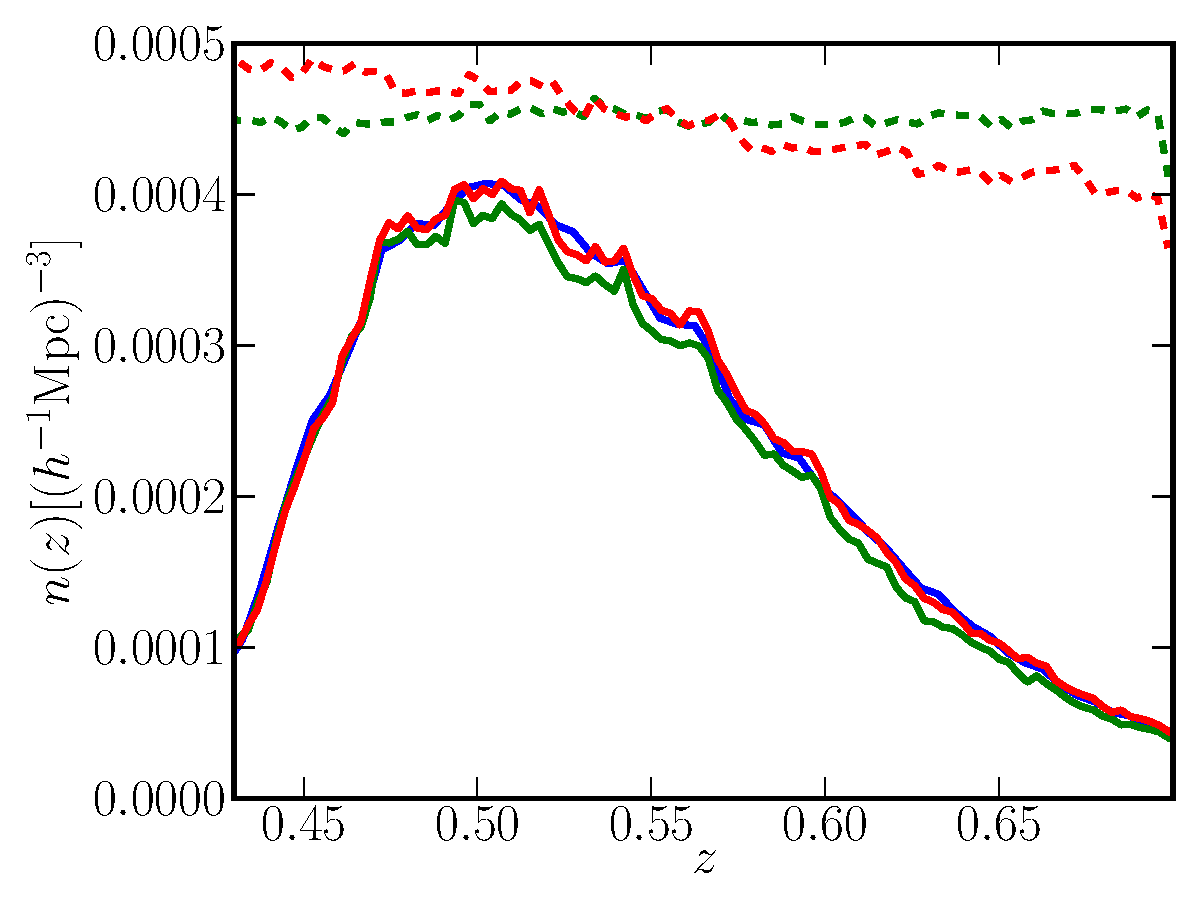
\includegraphics[width=0.5\columnwidth]{\lyxdot \lyxdot /Plots/nz_dr11_N}

\caption{\label{fig:nz_gal}A comparison of galaxy number densities before
fitting to DR11 (dashed lines) and after (solid lines). The blue solid
line is $n(z)$ from DR11 (North) in Ref.~\cite{2013arXiv1303.4666A}.
The green and red lines are from the mocks at $z=0.55$ and the lightcone
output respectively. The HOD parameters used to generate the mock
catalogs can be found in text.}
\end{figure}


\textcolor{red}{NOTE: not clear what the point of this figure is}

\begin{figure}
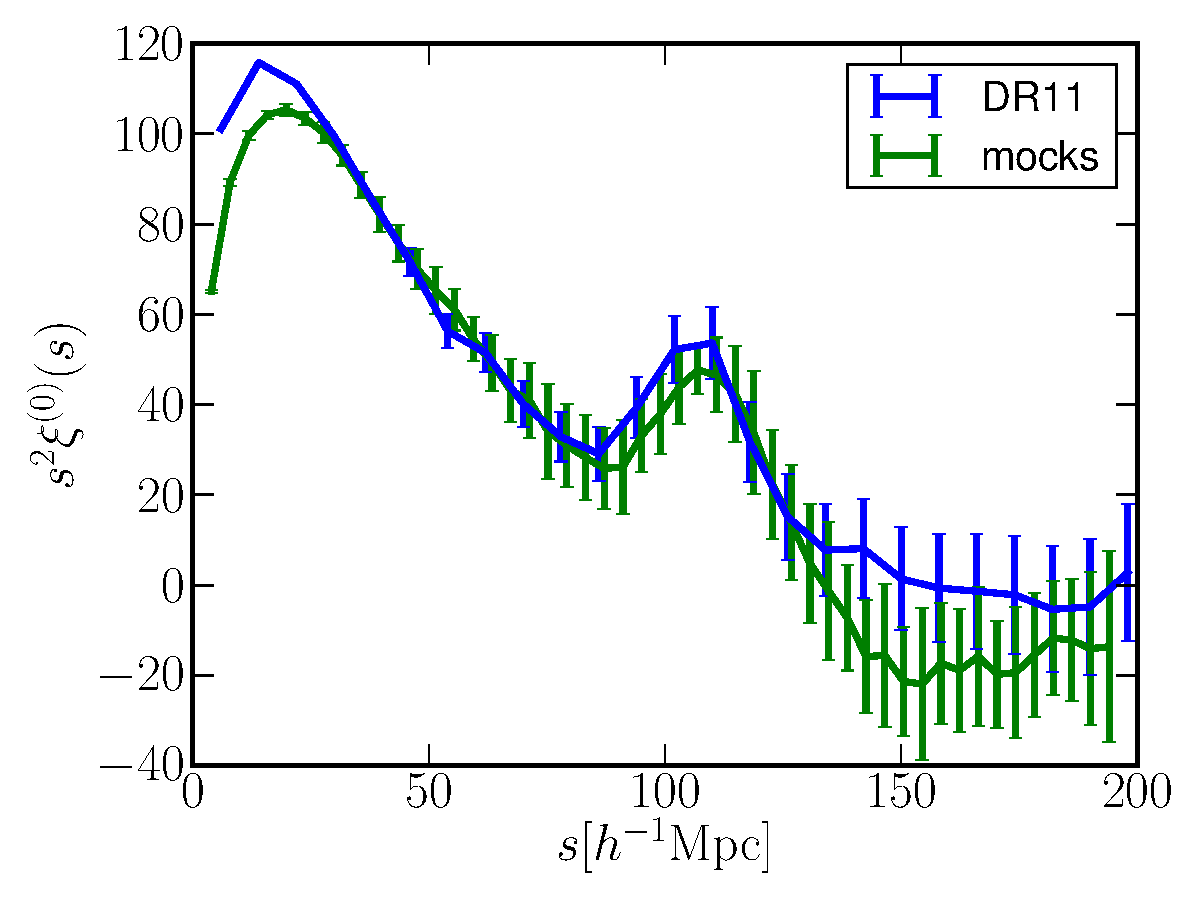
\includegraphics[width=0.5\columnwidth]{\lyxdot \lyxdot /Plots/xi0_obs}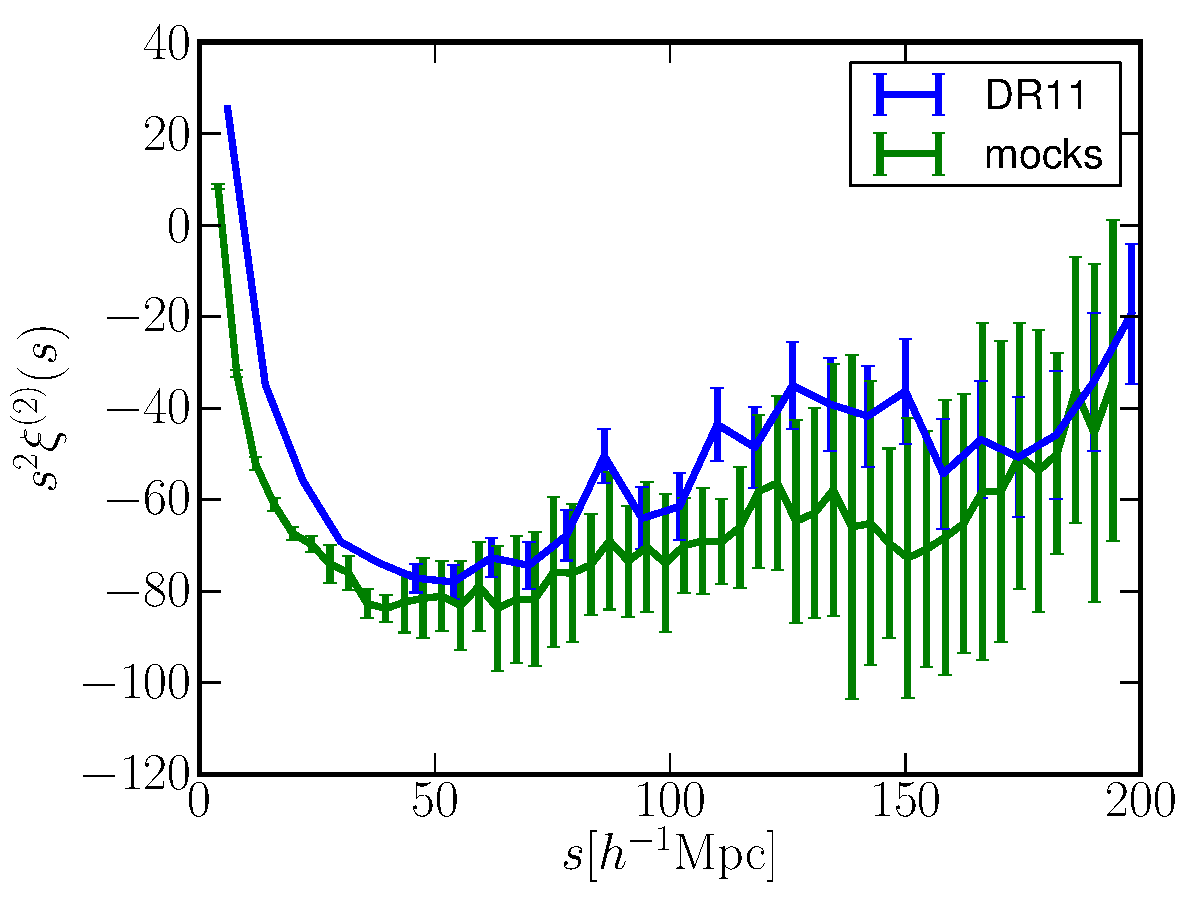
\includegraphics[width=0.5\columnwidth]{\lyxdot \lyxdot /Plots/xi2_obs}

\caption{\label{fig:xis}Correlation function monopoles $\xi^{(0)}(s)$ (left)
and quadrupoles $\xi^{(2)}(s)$ (right) of the mocks (green) and DR11
in Ref.~\cite{2013MNRAS.428.1036M} (blue) at $z=0.55$. The HOD
parameters used to generate the mock catalogs can be found in text.}
\end{figure}


\textcolor{red}{NOTE: need a better discussion of these results in
the text}


\section{Discussion}

Precision required for current and future galaxy spectroscopic surveys
to test the expansion and structure formation histories of the Universe
requires an accurate understanding of systematic effects. In this
paper we have presented a quantitative study of the impact of time
step sizes on the halo and matter density fields. Our code has two
adjustable time stepping parameters - a global time step and a number
of sub-cycles (responsible for a particle-particle interactions) to
track that particle trajectories on small scales. We consider cases
where we increase the length of each time step by factors of 1.5 and
3 respectively, as well as reducing the number of sub-cycles. Our
fiducial choice is to use using 300 global time steps corresponding
to $\Delta a(z)=0.003$ and 2 sub-cycles (increasing the length of
the global time step by a factor of 1.5 and that of the sub-cycles
by a factor of 2.5), resulting in a reduction of the simulation run
time by 4 times less. We keep the mass resolution constant; the results
here are based on a particle mass of $6.86\times10^{10}h{\rm M_{\odot}}$.We
summarize the key results below:

(a) The halo masses tend to be underestimated in these cases, as one
might expect because reducing the number of time steps produces halos
with less substructure and a more diffuse distribution of mass. However,
this trend may be calibrated with smaller simulations and corrected,
recovering the halo masses to 98\%. The halo mass function is correctly
recovered fully for masses above $10^{12.7}h^{-1}{\rm M_{\odot}}$
corresponding to 100 particles. Note that we run the halo finder with
identical parameters as in the full resolution runs. It may however
be possible to get similar results by changing the parameters of the
halo finder, as was done in \cite{2013MNRAS.428.1036M}.

(b) \textcolor{black}{The halo positions and velocities are recovered
with a scatter of $0.08[h^{-1}{\rm Mpc}]$ and $12.8[{\rm km/s}]$
respectively for the simulation of our fiducial choice. }

(c) The clustering of these halos is correctly recovered to better
than 1\% on scales below $k<1[h{\rm Mpc^{-1}]}$ in real-space and
$k<0.5[h{\rm Mpc^{-1}}]$.

(d) We find that the number of sub-cycles makes almost no difference
to any of our final results.

\textcolor{black}{We also consider the redshift sampling required
to construct light cone outputs. We first compare the distances for
the halos at different redshifts before and after shifting their positions
from one redshift to the another. Moving halos over a $\Delta z=0.1$
interval correctly reduces the standard deviation of those distances
from $0.25[h^{-1}{\rm Mpc}]$ to}\textcolor{red}{{} }\textcolor{black}{$0.09[h^{-1}{\rm Mpc}]$.
Moreover, the power spectra are correctly recovered to better than
1\% for $k<0.5[h{\rm Mpc^{-1}]}$ for $\Delta z=0.25$. This worsens
in redshift space to 2\% up to $k<0.2[h{\rm Mpc^{-1}]}$.}\textcolor{red}{{}
}\textcolor{black}{The agreement is, however, improved to 1\% for
$k<1[h{\rm Mpc^{-1}]}$ by using the velocity scaled by the relative
scale factor between the snapshot and the true redshift. Our fiducial
choice to construct light cone outputs is $\Delta z=0.05$.}

This work is a natural extension of the approaches described in \cite{2014MNRAS.439L..21K,2014MNRAS.437.2594W,2014arXiv1409.1124C,2013MNRAS.428.1036M,2014arXiv1401.4171M}.
The primary goal for those papers was to generate the large numbers
of simulations required for estimating covariance matrices. We quantify,
in detail, the impact of size of the time step on large scale observables;
our suite of simulations are better designed for testing for systematic
errors in theory and analysis techniques. As a proof of principle,
we present a set of eight full BOSS (both North and South Galactic
caps simultaneously) simulations. The time savings presented in this
paper allowed to extend this to 50 simulations, across a range of
cosmologies. These results from these will be presented in future
publications.


\section*{Acknowledgement}

TS and NP are supported by a DOE Early Career Grant. This work was
supported in part by the facilities and staff of the Yale University
Faculty of Arts and Sciences High Performance Computing Center, and
by resources at the National Energy Research Scientific Computing
Center. TS would like to thank Andrew Szymakowski for useful discussions.
This research used resources of the National Energy Research Scientific
Computing Center, a DOE Office of Science User Facility supported
by the Office of Science of the U.S. Department of Energy under Contract
No. DE-AC02-05CH11231. Argonne National Laboratory's work was supported
under U.S. Department of Energy contract DE-AC02-06CH11357.

\bibliographystyle{JHEP}
\bibliography{bigsims}

\end{document}
